\documentclass[biblatexieee]{kclthesis}

\usepackage[intoc]{nomencl}
\usepackage[toc, acronym]{glossaries}

\title{Argument Mining on Social Media}
\author{Danielius Marciukovas}
\modulecode{7CCSMPRJ}
\department{Department of Informatics}
\submissiontitle{Individual Project Submission 2018/19}
\studentnumber{1844311}
\programme{MSc Web Intelligence}
\supervisor{Josh Murphy}
\wordcount{1205}

\makenomenclature
\makeglossaries

\begin{document}
\pagenumbering{gobble}

\maketitle

%%%%%% empty page after main page.
\newpage
\thispagestyle{empty}
\mbox{}
\newpage

%%%%%% Abstract
\section*{Abstract}
Lorem ipsum dolor sit amet, consetetur sadipscing elitr, sed diam nonumy eirmod tempor invidunt ut labore et dolore magna aliquyam erat, sed diam voluptua. At vero eos et accusam et justo duo dolores et ea rebum. Stet clita kasd gubergren, no sea takimata sanctus est Lorem ipsum dolor sit amet. Lorem ipsum dolor sit amet, consetetur sadipscing elitr, sed diam nonumy eirmod tempor invidunt ut labore et dolore magna aliquyam erat, sed diam voluptua. At vero eos et accusam et justo duo dolores et ea rebum. Stet clita kasd gubergren, no sea takimata sanctus est Lorem ipsum dolor sit amet. 

%%%%%% Table of contents
\pagenumbering{roman}
\setcounter{tocdepth}{4}
\tableofcontents
\newpage

%%%%%%%%%%%%%%%%%%%%%%%%%%%%%%%%%%%%%%%%%%%%%%%%%%%%
%\thispagestyle{empty}
\listoffigures
\listoftables
\lstlistoflistings
\newpage
\mbox{}\newline\vspace{10mm} \mbox{}\LARGE
%
{\bf Acknowledgements} \normalsize \vspace{5mm}

I would like to thank my supervisor for providing me valuable support and feedback all throughout the year since I met him. He was helpful in guiding me in the right direction when I needed it and able to provide clearance on any matter whenever I had any concerns or questions. 

\fancyhead{}
\fancyfoot{}
\pagestyle{fancy} 
\fancyhead[R,L]{\sffamily\small \thepage}
\fancyhead[LO]{\sffamily\small \nouppercase{\rightmark}}

%\fancyhead[RO,L]{\sffamily\small \thepage}
%\fancyhead[LO,RE]{\sffamily\small \nouppercase{\rightmark}}
\renewcommand{\headrulewidth}{0.4pt}
\renewcommand{\footrulewidth}{0.0pt}

%%%%%%%%%%%%%%%%%%%%%%%%%%%%%%%%%%%%%%%%%%%%%%%%%%%%
%%%%%% Main content
\pagenumbering{arabic}
%\section{Feedback}
For Introduction:
\begin{itemize}
    \item There is a bit too much technical detail for the introduction. You should aim your introduction to a computer scientist that doesn't know about argumentation. So spend some time to explain the general idea of argumentation before getting into argument mining.

    \item The information is quite dense. Spend some more time to explain the concepts you are stating. For example, in paragraph 2, in the list of difficulties you could explain each of these in their own sentence.

    \item What is an argument attack? What is the context of an argument? What makes social media different to legal documents? Make sure your reader understand what you mean by these points.

    \item The motivation in the third paragraph is good. I would move this above the explanation of why the problem is challenging. 

    \item You might want to put each of these in their own subsection.
\end{itemize}
\section{Introduction}
\subsection{Overview} 
 Argumentation is a subject that studies processes involved in reasoning and the structure of reason itself. It is a field that encompasses and spans across multiple other fields, most notably language, philosophy, psychology, logic and has recently transcended into \gls{ai}. This is because \gls{ai} provides the ability to conjoin mental reasoning models and mathematical models for automated reasoning \citep{Lippi2016ArgumentationMS}. The applications of argument models within computer science and \gls{ai} are vast in possibilities. The ability to view and model such arguments provides important insight into how humans reason about different claims, how the claims are supported or disagreed with. Given an argument model applied to a discussion forum or a debate, this would provide an opportunity to understand more deeply and extract points of view that carry the most weight \citep{Cocarascu2017MiningBA}. Subsequently, it would be possible to analyse the flow of the discussion and see how the positions taken within the debate change over time as new arguments are introduced. On the other hand, same argument models can also allow us to investigate how a certain perception of something (review, feedback, etc.) can be altered \citep{ApproxToTruth}. Also, this is a hot topic with regards to ethics within the \gls{ai} system. The decisions that we delegate to \gls{ai} to make, have to be verifiable, thus meaning the system has to be able to show the arguments that it worked with and how the consensus on the decision was made. All in all, industries that would benefit would be law, politics and political debates, reviews and marketing, social media platforms to name a few.
 
\subsection{Argument Mining}
 
 \gls{am} is an intensive research field focused on automatically extracting arguments and their interrelationships from text documents. Due to recent technological advancements in other fields such as \gls{ai}, \gls{nlp} and \gls{ml}, this is becoming more and more possible. Moreover, internet provides unlimited amounts of data to analyse and extract arguments from with accessibility to websites such as Facebook, Twitter, Wikipedia Talks, Reddit and other popular social media pages 
 
 Unfortunately, this is not easy to do. The definition of argument is hard to express in mathematical or computer science terms. First of all, there are no limits as to how long an argument should be. An argument, depending on the corpora, can be a part of a sentence or the whole document could be one big argument backed by many smaller arguments within it (e.g. a certain law article is broken down into sections, which are then broken down into paragraphs and so on). Secondly, the nature of the argument has to be understood, to determine whether it is supporting any other argument, or attacking it. An argument is considered to be a supporting argument if it is on point with the view made by the previous original argument. Conversely, going back to the law example, an attack to the argument could be considered in the sense of an exception that is stated within the law, where the law doesn't apply. 
 
 These points coupled together mean that argument classification problem is dependent on meaning of the argument itself, which makes this also a \gls{nlp} problem. Context or topic of the corpora matters a lot as well, because of language stylistic differences. It is no surprise that legal documents entail a more precise syntactical text structure, due to the nature of the industry requiring concrete descriptions to cover and exclude very specific cases of application. On the other hand, texts found in social media are of a more diverse linguistic composition, where messages posted by users can be very conversational or carry a meaning that is only understood by a certain group of people (e.g. abbreviations, specific background required).

\subsection{Project Aims and Objectives} 
 The aim of this project is to gain an up to date knowledge of current trends and advancements within the field of argumentation mining, to create a tool that given a specific chain of arguments in text form would analyse such arguments and construct an \gls{af} displaying the winning or most convincing arguments, and to contribute to the research community by explaining views and sharing ideas pertaining to the problem at hand.

\subsection{Background and Literature Survey} \label{sub:background}

This part is for literature review.

% It gives an overall picture about the work with a clear review of the relevant literature.  The background of the project should be given.  What have been done to deal with the problem should be stated clearly.  The pros and cons of various existing algorithms and approaches should be stated as well.  Differences between your proposed method and the existing ones should be briefly described. 

%The following links may help on the literature review: IEEE Xplore digital library: a resource for accessing IEEE published scientific and technical publications. (You must be with King's network to get access to the digital library) ScienceDirect.com: an electronic database offering journal papers not published by IEEE (You must be with King's network to get access to the database)

\section{Background Theories} 

This section describes what the reader has to know in order to understand my project.
\section{Main Result}
The chapter reports the contribution of your work.  For example, it could contain the following sub-sections to summarise the contribution of the project: Theoretical Development, Analysis and Design, Implementation and Experimental Work, Results, Observation and Discussion.

\subsection{Maths}
\begin{equation}\label{eq:BS}
\frac{\D S_t}{S_t} = r \D t + \sigma \D W_t,
\qquad S_0>0,
\end{equation}

The equation $\sigma = m a$ follows easily~\cite{Doe11}.


\subsection{Glossary and acronyms}

\Glspl{Linux} and other Unix operating systems are better then Windows because they support \gls{lvm} out of the box~\cite{Joh11}\insertref{A ref is missing here}. 

\subsection{Figures}
Here is an example~\cite{JohSil05} of how to inserta picture:

\begin{figure}[!ht]
\centering
\subfigure{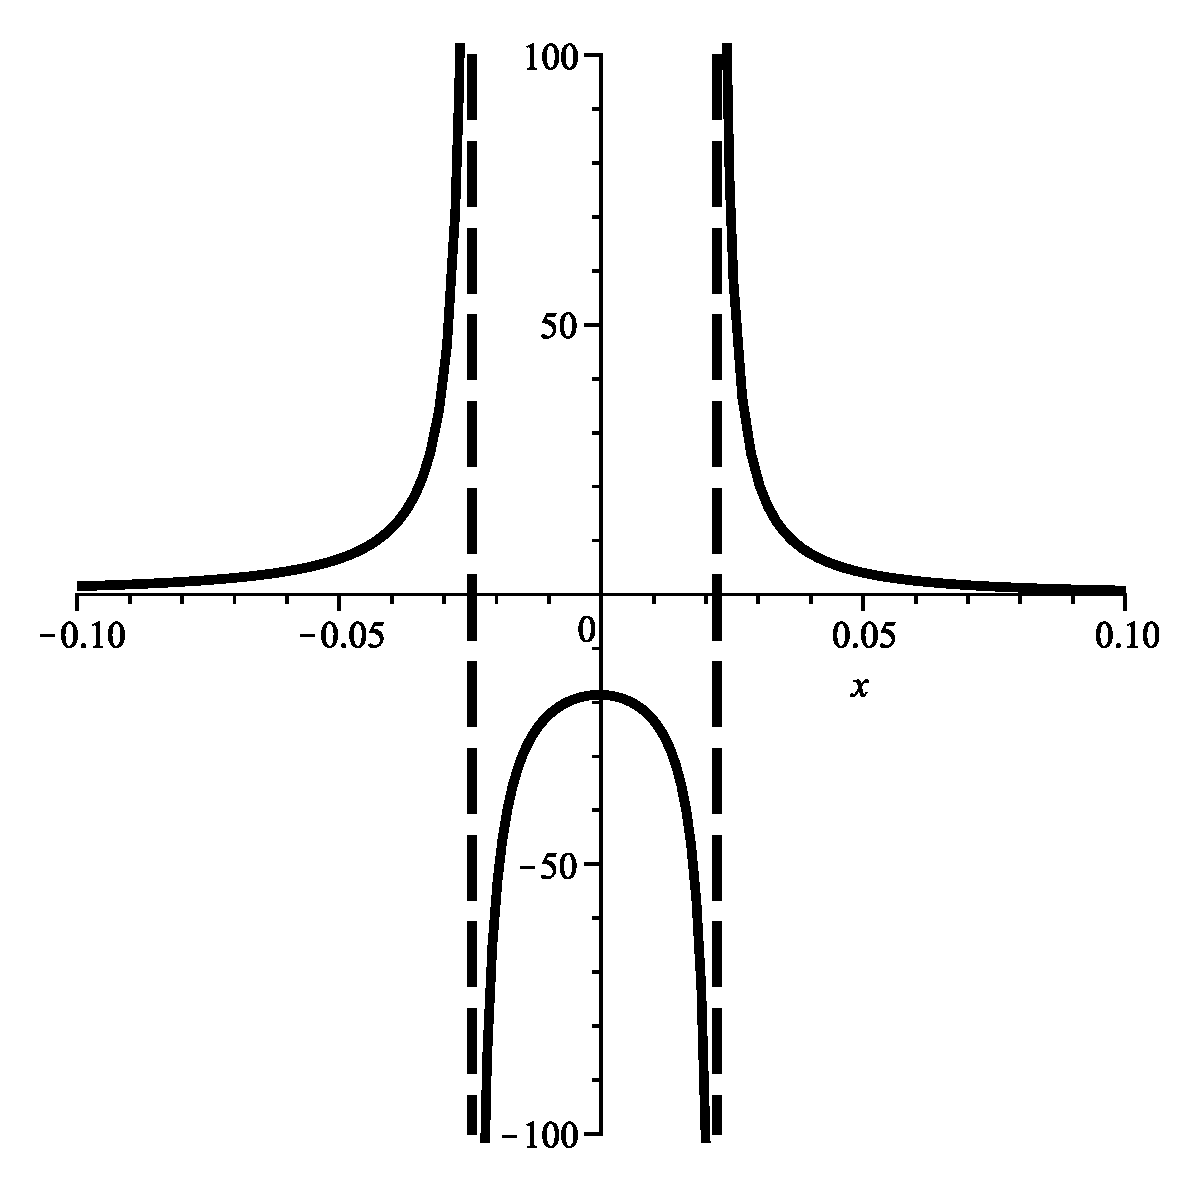
\includegraphics[scale=0.2]{figures/Picture.eps}}
\caption{This is the caption for the figure.}
\label{fig:Pict}
\end{figure}


\begin{figure}[!ht]
\centering
\missingfigure{If you know there will be a figure, but you still need to create it.}
\caption{This is the caption for the figure which is not even present.}
\label{fig:PictMis}
\end{figure}


Lorem ipsum dolor sit amet, consetetur sadipscing elitr, sed diam nonumy eirmod tempor invidunt ut labore et dolore magna aliquyam erat, sed diam voluptua. At vero eos et accusam et justo duo dolores et ea rebum. Stet clita kasd gubergren, no sea takimata sanctus est Lorem ipsum dolor sit amet. Lorem ipsum dolor sit amet, consetetur sadipscing elitr, sed diam nonumy eirmod tempor invidunt ut labore et dolore magna aliquyam erat, sed diam voluptua. At vero eos et accusam et justo duo dolores et ea rebum. Stet clita kasd gubergren, no sea takimata sanctus est Lorem ipsum dolor sit amet.\todo{This is a small Todo, please take care!}

or two side-by-side pictures:

\begin{figure}[!ht]
\centering
\subfigure{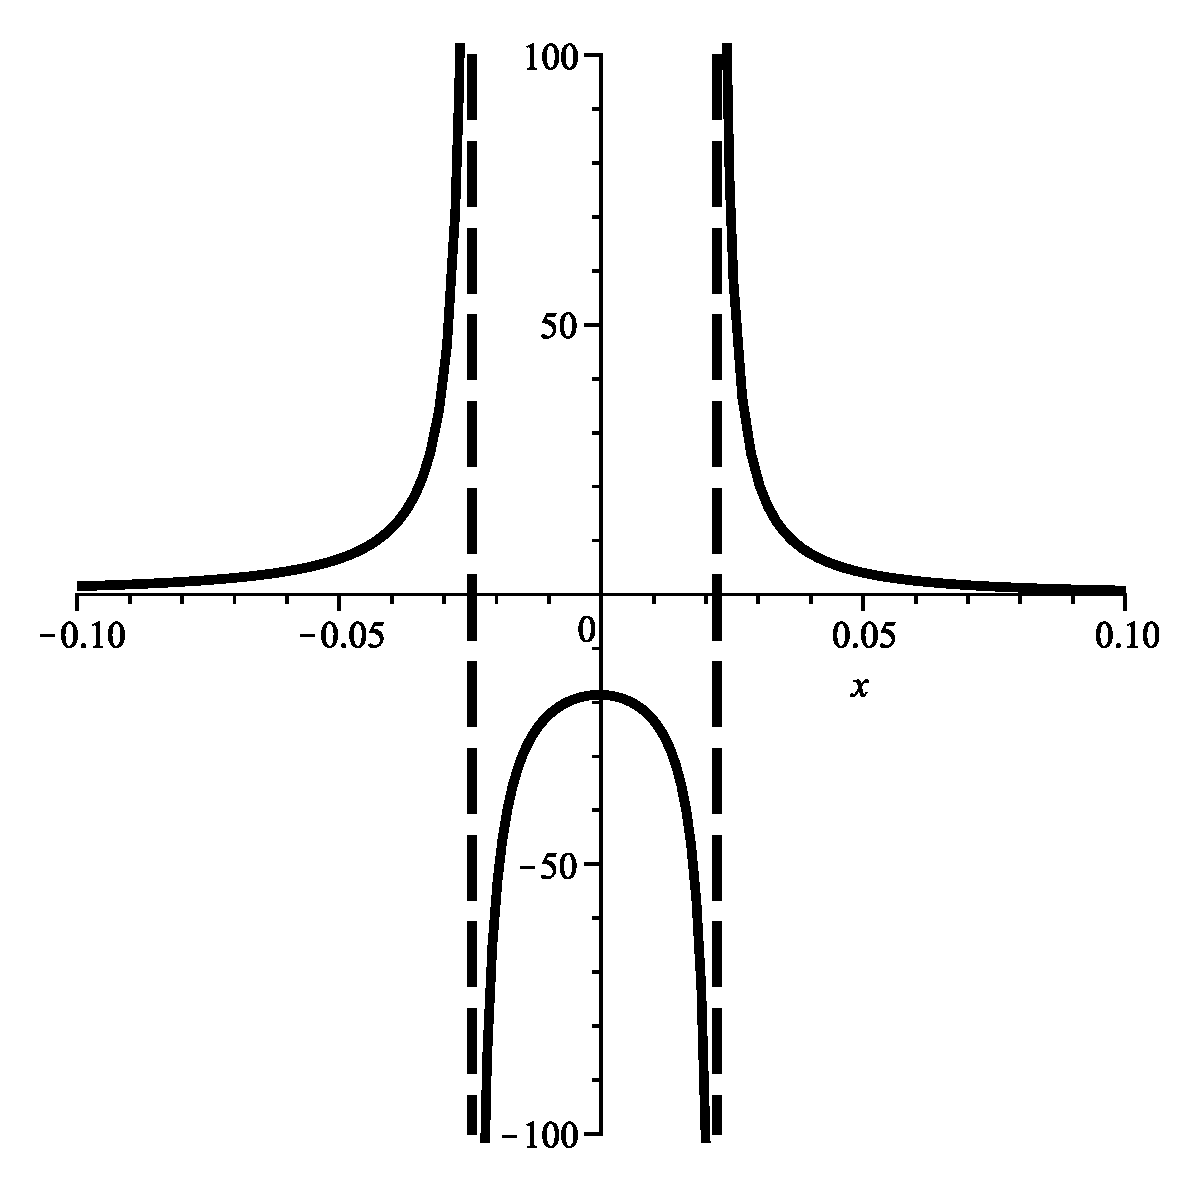
\includegraphics[scale=0.3]{figures/Picture.eps}}
\hspace{15pt}
\subfigure{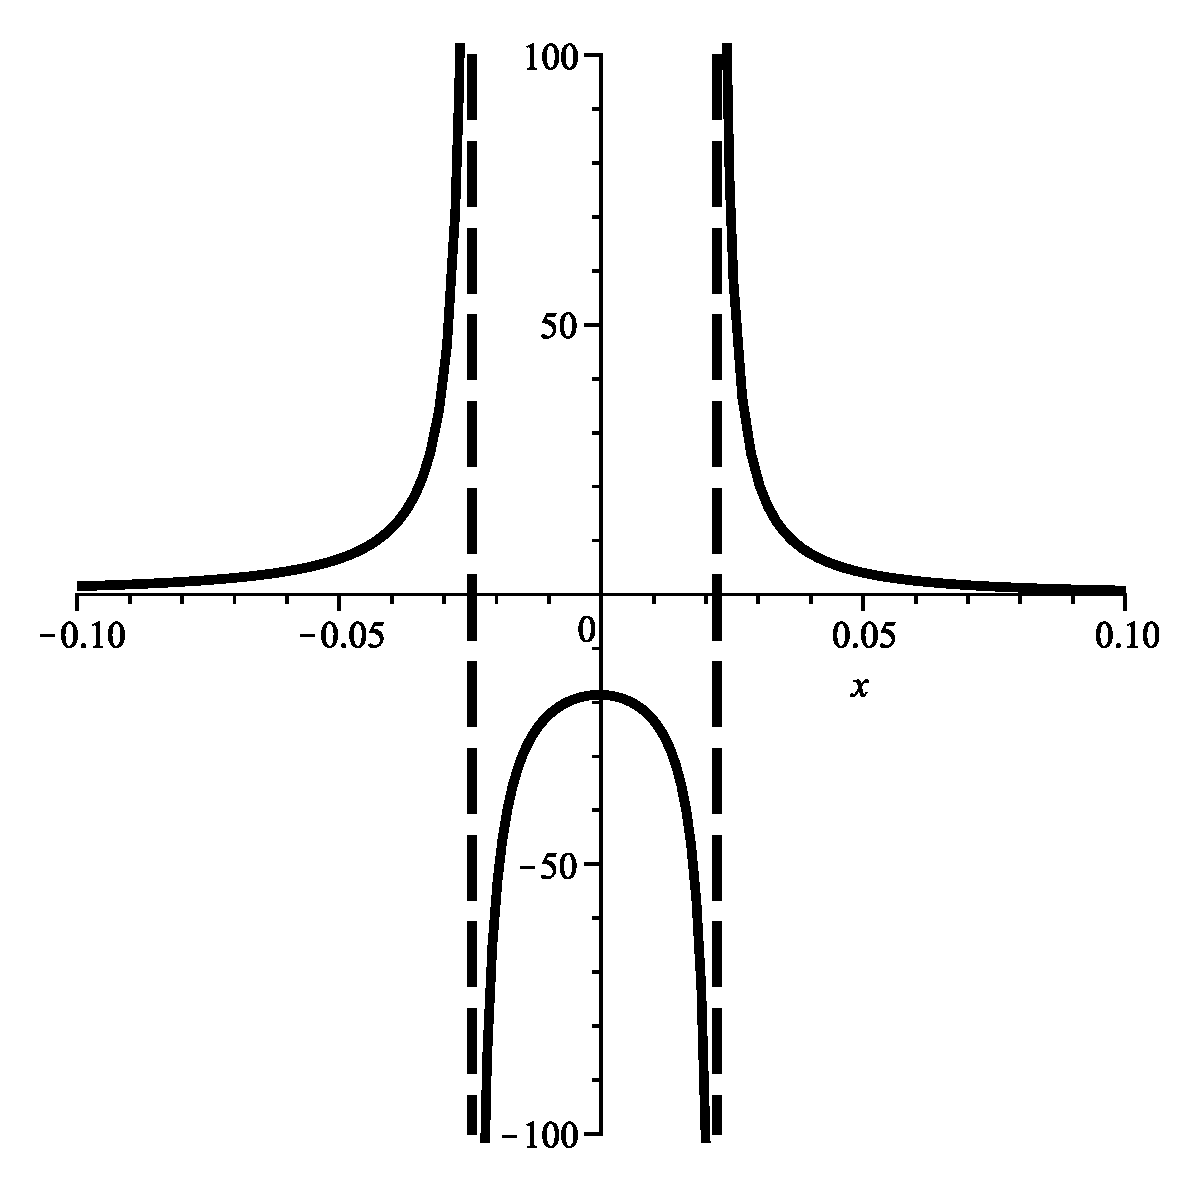
\includegraphics[scale=0.3]{figures/Picture.eps}}

\caption{Another caption}
\label{fig:Pict2}
\end{figure}



\subsection{Table}
Lorem ipsum dolor sit amet, consetetur sadipscing elitr, sed diam nonumy eirmod tempor invidunt ut labore et dolore magna aliquyam erat, sed diam voluptua. At vero eos et accusam et justo duo dolores et ea rebum. Stet clita kasd gubergren, no sea takimata sanctus est Lorem ipsum dolor sit amet. Lorem ipsum dolor sit amet, consetetur sadipscing elitr, sed diam nonumy eirmod tempor invidunt ut labore et dolore magna aliquyam erat, sed diam voluptua. At vero eos et accusam et justo duo dolores et ea rebum. Stet clita kasd gubergren, no sea takimata sanctus est Lorem ipsum dolor sit amet\explainindetail{This needs further explanation}.
\begin{table}[!ht]
	\centering
	\begin{tabular}{|l|rl|}
		\hline
		Something & Someother & Thing \\
  		Seems & to be & good\\
  		\hline
  	\end{tabular}
  	\caption{Random data for a table.}
\end{table}

Lorem ipsum dolor sit amet, consetetur sadipscing elitr, sed diam nonumy eirmod tempor invidunt ut labore et dolore magna aliquyam erat, sed diam voluptua. At vero eos et accusam et justo duo dolores et ea rebum. Stet clita kasd gubergren, no sea takimata sanctus est Lorem ipsum dolor sit amet. Lorem ipsum dolor sit amet, consetetur sadipscing elitr, sed diam nonumy eirmod tempor invidunt ut labore et dolore magna aliquyam erat, sed diam voluptua. At vero eos et accusam et justo duo dolores et ea rebum. Stet clita kasd gubergren, no sea takimata sanctus est Lorem ipsum dolor sit amet.


\section{Model calibration}
\subsection{What is calibration?}
Here is an example of a matrix\cite{website:fermentas-lambda} in $A\in\mathcal{M}_n(\RR)$:
$$
A = 
\begin{pmatrix}
a_{11} & a_{12} & \ldots & a_{1n}\\
a_{21} & \ddots & \ddots  & \vdots\\
\vdots &  \ddots & \ddots  & \vdots\\
a_{n1} &  \ldots &  \ldots & a_{1n}.
\end{pmatrix}
$$

\subsection{Numerical methods for calibration}
...



\section{Conclusion} \label{conclusions}
    This section briefly summarises what has been achieved throughout the project. Analysis performed on two government systems used by English speaking countries showcase interesting social tendencies how the public treats and reacts to opposing parties. It is sufficient to say that this is only the tip of the iceberg and there are many different topics that can be explored in the same manner, not only politics as was chosen here.
    
    The contribution to research community is substantial. The trained classifier is in line with expected performance given the circumstances of hardware limitations, and the overall software is a stepping stone to combining argument mining, extraction, relation detection and framework analysis into one coherent process, with high hopes of becoming an advanced system capable of handling multiple models and multiple social media platforms.
\newpage

\newacronym{ai}{AI}{Artificial Intelligence}
\newacronym{nlp}{NLP}{Natural Language Processing}
\newacronym{ml}{ML}{Machine Learning}
\newacronym{te}{TE}{Textual Entailment}
\newacronym{af}{AF}{Argumentation Framework}
\newacronym{aaf}{AAF}{Abstract Argumentation Framework}
\newacronym{baf}{BAF}{Bipolar Argumentation Framework}
\newacronym{am}{AM}{Argumentation Mining}
\newacronym{edits}{EDITS}{Edit Distance Textual Entailment Suite}
\newacronym{api}{API}{Application Programming Interface}
\newacronym{eop}{EOP}{Excitement Open Platform}
\newacronym{rnn}{RNN}{Recurrent Neural Network}
\newacronym{lstm}{LSTM}{Long Short-Term Memory}
\newacronym{snli}{SNLI}{Stanford Natural Language Inference}
\newacronym{ram}{RAM}{Rapid-Access Memory}
\newacronym{cpu}{CPU}{Central Processing Unit}
\newacronym{gpu}{GPU}{Graphics Processing Unit}
\newacronym{vram}{VRAM}{Video Rapid-Access Memory}
\newacronym{csv}{CSV}{Comma-Separated Values}
\newacronym{os}{OS}{Operating System}
\newacronym{glove}{GloVe}{Global Vectors for Word Representation}
\newacronym{ddos}{DDoS}{Distributed Denial of Service}
\newacronym{url}{URL}{Uniform Resource Locator}
%\newglossaryentry{pi}{name={\ensuremath{\pi}}, description={ratio of circumference of circle to its diameter}, sort=pi}
%\newglossaryentry{Linux}{name=Linux,description={is a generic term referring to the family of Unix-like computer operating systems that use the Linux kernel}, plural=Linuces}
\printglossaries

\newpage

%%%%% References
% For KCL Harvard V1: \bibliographystyle{kclharvardv1}
% For natbib-ieee: 
% \bibliographystyle{ieeetr}
% \bibliography{bibs/bibliography}
% For biblatex-ieee:
\nocite{*}
\printbibliography

%%%%% Declaration
%\thispagestyle{empty}


\mbox{}\newline\vspace{10mm} \mbox{}\LARGE
%
{\bf Declaration} \normalsize \vspace{5mm}

I declare that this thesis is the solely effort of the author.
I did not use any other sources and references than the listed ones. I have marked all contained direct or indirect statements from other sources as such.

Neither this work nor significant parts of it were part of another review process.
I did not publish this work partially or completely yet.
The electronic copy is consistent with all submitted copies.

\bigskip
\bigskip
\bigskip
\bigskip


Signature and date: 






%%%%% Appendix 
\appendix

\section{Review of stochastic calculus}
\subsection{Riemann integration}


\subsection{The It\^o integral}




\end{document}
